\documentclass[11pt,a4paper]{article}
\usepackage[T1]{fontenc}
\usepackage{lmodern}
\usepackage[margin=2.4cm]{geometry}
\usepackage{amsmath,amssymb}
\usepackage{graphicx}
\usepackage{booktabs}
\usepackage{placeins}
\usepackage{microtype}
\usepackage{enumitem}
\usepackage[font=small,labelfont=bf]{caption}
\usepackage[dvipsnames]{xcolor}
\usepackage[colorlinks=true,linkcolor=MidnightBlue,urlcolor=MidnightBlue]{hyperref}

\graphicspath{{../../analysis/figs/}}
\setlist{itemsep=2pt,topsep=4pt}
\newcommand{\CL}{C_L}
\newcommand{\figw}{\linewidth}

\title{How many terms does the steady lift curve need?\\[2pt]
\large NACA0012, 2D laminar, Re = 100, 500, 1000, 2000}
\author{Steady-lift fitting report}
\date{6 October 2026}

\begin{document}
\maketitle

\noindent
This report summarises what we learned by fitting simple formulas to the steady lift
curve $\CL(\alpha)$ of the NACA0012 at four Reynolds numbers. It is written to be read
without a background in Lasso regression or orthogonal polynomials: those ideas are
explained in Section~\ref{sec:methods}, in plain terms, at the point where they are
needed.

\section{Highlights}

\begin{enumerate}[leftmargin=*]
\item \textbf{Below the shedding angle, the lift curve is essentially
  $\CL \approx a_1\theta + a_3\theta^3$} ($\theta$ = angle of attack in radians).
  At Re = 500, 1000 and 2000, over $0$--$8^\circ$, every method we tried keeps exactly
  these two terms as the important ones.

\item \textbf{The cubic correction grows steadily with Reynolds number.} The higher
  the Re, the earlier and harder the lift curve bends over. The size of the bend,
  $|a_3|$, follows $|a_3| \approx 0.48\,\mathrm{Re}^{0.66}$ from Re = 100 to 2000.
  The linear slope $a_1$ hardly changes (2.9--3.3 per radian, about $\pi$).

\item \textbf{Re = 100 is almost a straight line} over $0$--$8^\circ$, and
  \textbf{Re = 2000 already needs a third term} ($\theta^5$), because its lift curve
  flattens out before $8^\circ$.

\item \textbf{The best way to write the fit is in Legendre polynomials, not powers of
  $\theta$.} Powers of $\theta$ look almost identical to each other over a small
  angle range, so their coefficients are unstable. Legendre coefficients are stable
  and can be compared across Re directly (Section~\ref{sec:legendre}).

\item \textbf{The steady solution is not what the flow does above the shedding angle.}
  At Re = 2000, $\alpha = 9.5^\circ$, the time-accurate simulation sheds vortices with
  mean $\CL = 0.441$, which is 79\,\% above the steady value of 0.247. The whole
  oscillation sits above the steady value.
\end{enumerate}

\section{What to be skeptical about}

\begin{itemize}[leftmargin=*]
\item \textbf{The meshes are not verified at Re = 100, 1000 or 2000.} Only Re = 500 has
  a mesh-independence study. The other meshes use the same layout, with the first cell
  height rescaled with Re. Re = 2000 is the most exposed.

\item \textbf{``Below the shedding angle'' is assumed, not measured, for most cases.}
  We measured the shedding onset precisely only at Re = 500 ($11.46^\circ$). At
  Re = 1000 it lies between $8^\circ$ and $10^\circ$. At Re = 2000 we only know that
  $9.5^\circ$ sheds. Shedding could start lower, inside our fit ranges.

\item \textbf{The power law $|a_3| \propto \mathrm{Re}^{0.66}$ is four points on one
  family of meshes.} It is an observation, not a derived scaling law. Using the
  $0$--$8^\circ$ range instead of $0$--$6^\circ$ changes the exponent from 0.66 to 0.60.

\item \textbf{Lasso's choice of terms depends on our settings.} With a fixed penalty,
  the terms it keeps change with the angle range we fit. It is a useful screening tool,
  not proof that the physics ``contains'' exactly those terms
  (Section~\ref{sec:lasso}).

\item \textbf{The data have no noise, so ``goodness of fit'' means something
  different here.} CFD gives the same answer every time. The leftover error of a fit
  is a modelling error, not random scatter, and it can be pushed down almost to the
  output precision ($\sim 10^{-7}$ in $\CL$) by adding terms. Statistical tools that
  assume noise, such as cross-validation, therefore always prefer more terms.

\item \textbf{The unsteady Re = 2000 run is short.} It was stopped at
  $t \approx 30$, as soon as shedding was clear, after about 11 cycles. Its mean and
  amplitude are good to about $\pm 1\,\%$. It is not long enough for POD.

\item \textbf{2D laminar flow at Re = 2000} is an assumption of the whole campaign.
\end{itemize}

\section{Methods}
\label{sec:methods}

\FloatBarrier
\subsection{The simulations}

\begin{itemize}[leftmargin=*]
\item \textbf{Code and model.} OpenFOAM, incompressible, 2D, laminar, NACA0012 with
  chord 1 and free stream speed 1, so Re = $1/\nu$.
\item \textbf{Mesh.} One structured O-mesh per Reynolds number, 63\,360 cells, far
  field at radius 30 chords. Only the height of the first cell at the wall changes with
  Re, following the Blasius boundary-layer scaling $h_1 = 0.05/\sqrt{\mathrm{Re}}$.
\item \textbf{Angle of attack} is set by rotating the incoming flow, so the same mesh
  serves every angle.
\item \textbf{Steady solutions.} We solve the steady equations (the SIMPLE algorithm)
  at every angle from $0^\circ$ to $12^\circ$ in $0.5^\circ$ steps, plus 14, 16, 18 and
  $20^\circ$.
\item \textbf{Convergence is judged on the lift itself.} A case counts as converged
  when $\CL$ stops changing over the last 10\,\% of iterations. Above some angle the
  steady solver no longer settles and $\CL$ keeps oscillating between iterations; those
  cases are excluded from all fits.
\end{itemize}

\noindent
\textbf{An important subtlety.} The steady solver throws away the time derivative, so
it can converge to a solution that the real, time-dependent flow would leave
immediately. Above the shedding angle the steady solution still exists, but the flow
does not stay there. Section~\ref{sec:unsteady} shows this directly.

\begin{table}[htbp]
\centering
\caption{Where the steady solver stops settling.}
\begin{tabular}{rll}
\toprule
Re & steady solver converges & first angle where it oscillates \\
\midrule
100  & every angle, $0$--$20^\circ$ & none \\
500  & up to $20^\circ$ & $22^\circ$ \\
1000 & up to $12^\circ$ & $14^\circ$ \\
2000 & up to $9^\circ$ & $9.5^\circ$ \\
\bottomrule
\end{tabular}
\end{table}

\FloatBarrier
\subsection{Odd symmetry: why only odd powers}
\label{sec:odd}

The NACA0012 is symmetric: its upper and lower surfaces are mirror images. Turning it
to $-\alpha$ is the same as turning it to $+\alpha$ and flipping the picture upside down.
Flipping the picture reverses the lift. So
\[
  \CL(-\alpha) = -\CL(\alpha),
\]
which mathematicians call an \emph{odd} function. Figure~\ref{fig:sym} shows our
computed points and their mirror images.

A polynomial is odd only if it contains odd powers alone: $\theta$, $\theta^3$,
$\theta^5$, \dots. Even powers ($1$, $\theta^2$, $\theta^4$, \dots) give the same value
at $+\theta$ and $-\theta$, so they cannot appear in the true lift curve. In particular
there is no constant term: $\CL(0) = 0$.

Two practical consequences:
\begin{itemize}[leftmargin=*]
\item We only need to simulate positive angles. The negative side is known exactly.
\item If a fit ever picks an even power, that tells us about the fitting method, not
  about the flow. This happened: Lasso picked $\theta^4$ when allowed to
  (Section~\ref{sec:lasso}).
\end{itemize}

\begin{figure}[htbp]
\centering
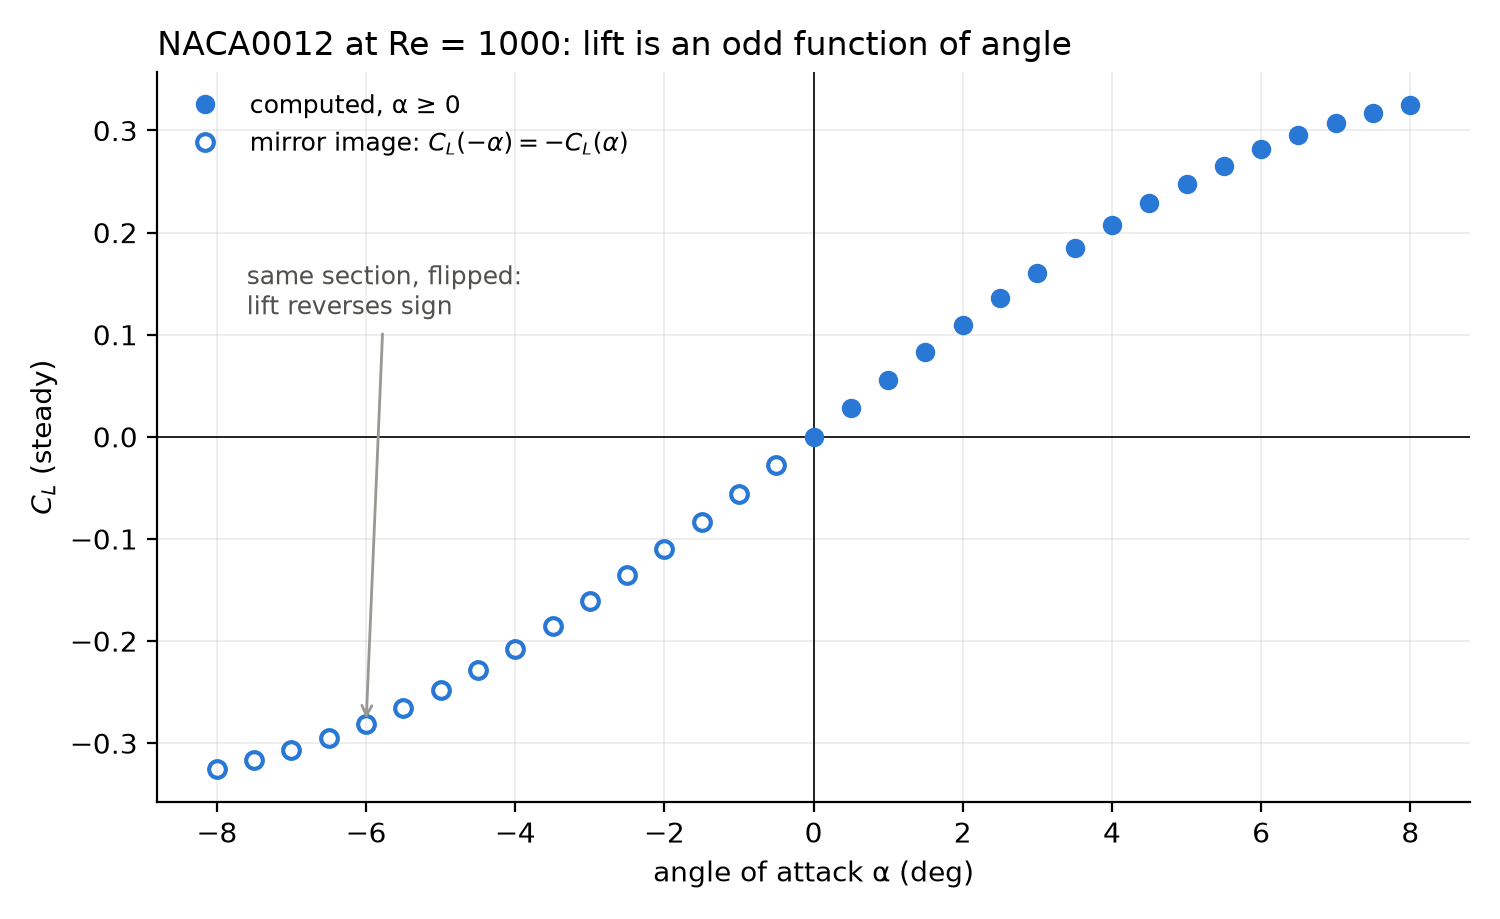
\includegraphics[width=0.72\linewidth]{partner_report/symmetry.png}
\caption{Computed lift at Re = 1000 for $\alpha \ge 0$ (filled) and its mirror image
(open). The two halves join smoothly through the origin.}
\label{fig:sym}
\end{figure}

\FloatBarrier
\subsection{Why powers of \texorpdfstring{$\theta$}{theta} are a poor set of building blocks}
\label{sec:lookalike}

A polynomial fit builds the lift curve out of ``building blocks'' ($\theta$,
$\theta^3$, \dots) and finds how much of each to use. That works well only if the
blocks look different from each other. Over our range, $0$ to $8^\circ$
($0$ to 0.14 radians), they do not (Figure~\ref{fig:look}, left):
\begin{itemize}[leftmargin=*]
\item $\theta$, $\theta^2$ and $\theta^3$ all start at zero and rise steadily. Scaled
  to the same end value, they differ only in how much they sag in the middle.
\item Their correlation over our data points is 0.91 to 0.99. A correlation of 1 would
  mean they are the same shape.
\item A straight line through the data already explains 93\,\% of $\theta^2$ and
  83\,\% of $\theta^3$. To a line fit, they are mostly the same thing as $\theta$.
\end{itemize}

When the blocks are this alike, many different mixtures produce nearly the same
curve. Then the fitted amounts become unstable: add a point or another term, and the
coefficients jump around and can change sign, even though the fitted \emph{curve}
hardly changes. The numerical measure of this is the \emph{condition number}, roughly
how much small changes in the data can be amplified in the coefficients. For the nine
powers $\theta^1$--$\theta^9$ on our data it is about $10^{12}$. For a well-behaved
fit it should be close to 1.

\begin{figure}[htbp]
\centering
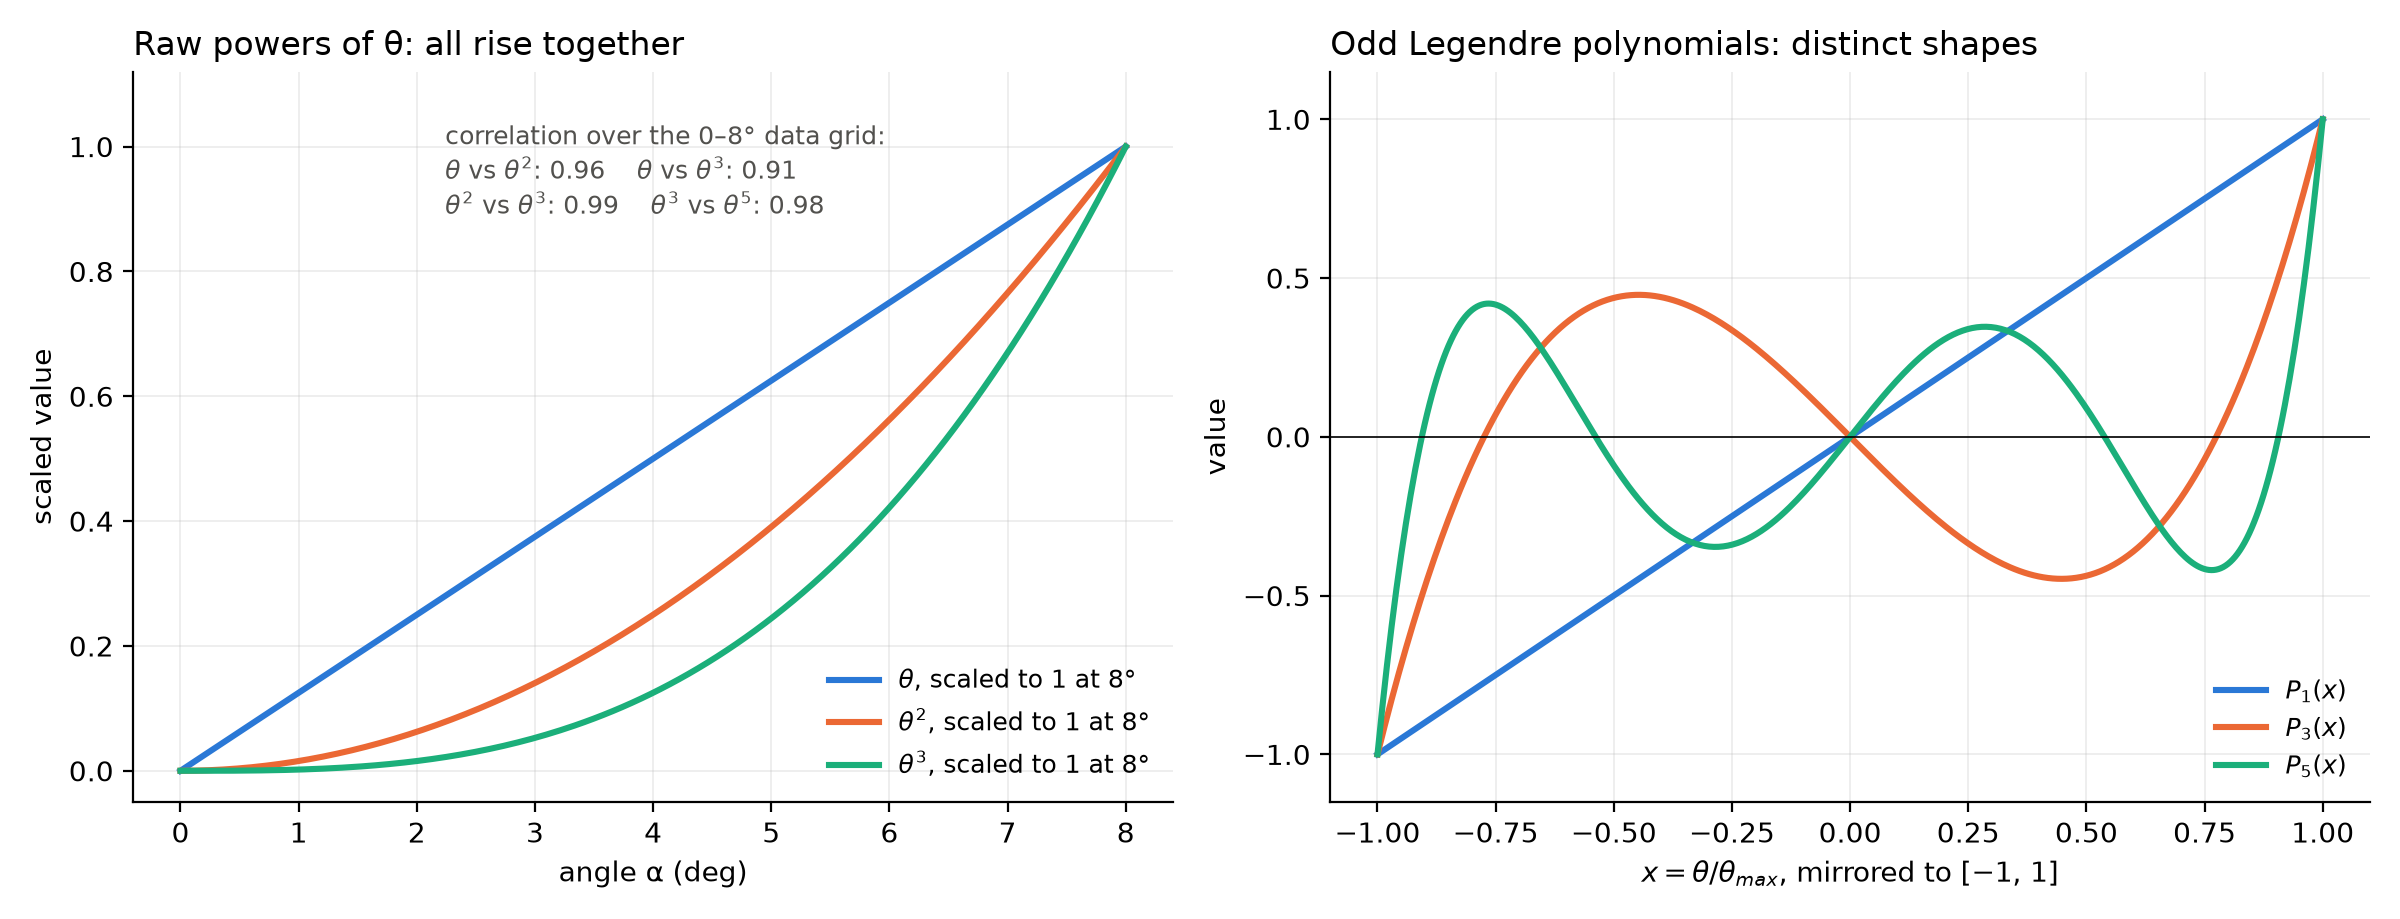
\includegraphics[width=\figw]{partner_report/lookalike.png}
\caption{Left: $\theta$, $\theta^2$, $\theta^3$ over $0$--$8^\circ$, each scaled to 1
at $8^\circ$. They all rise together and are hard for a fit to tell apart. Right: the
first three odd Legendre polynomials on the mirrored, rescaled range. Each has a clearly
different shape.}
\label{fig:look}
\end{figure}

\FloatBarrier
\subsection{Lasso: an automatic way to drop terms}
\label{sec:lasso}

\textbf{The idea.} An ordinary least-squares fit makes the error as small as possible
and uses every term you give it. Lasso adds a cost for every coefficient that is not
zero. It minimises
\[
  \underbrace{\text{(fit error)}}_{\text{be accurate}} \;+\;
  \lambda \times \underbrace{\textstyle\sum_k |\text{coefficient}_k|}_{\text{be simple}} .
\]
The ``penalty'' $\lambda$ sets the trade-off. Small $\lambda$ keeps almost every term.
Large $\lambda$ drives coefficients to exactly zero, so only the terms that earn their
cost survive. Before fitting, every term is rescaled to the same spread, so the penalty
treats them equally.

\textbf{What we did.}
\begin{itemize}[leftmargin=*]
\item Fit $\CL$ with candidate terms $\theta, \theta^3, \theta^5, \theta^7, \theta^9$
  (odd only, Section~\ref{sec:odd}), at $\lambda = 10^{-4}$, the value used in the
  original Re = 500 analysis.
\item Traced the \emph{coefficient path}: how each coefficient changes as $\lambda$ is
  slowly turned up from zero.
\item \textbf{Bootstrap check.} Refitted 500 times, each time on a random resample of
  the data points, and counted how often each term survived. A term kept in 100\,\% of
  resamples is a firm choice; one kept in 50\,\% is a coin toss.
\end{itemize}

\textbf{Its weakness here.} Because the powers of $\theta$ look so alike
(Section~\ref{sec:lookalike}), Lasso often has no firm reason to prefer one over
another. It then keeps whichever one happens to be slightly cheaper:
\begin{itemize}[leftmargin=*]
\item When even powers were allowed, it picked $\theta^4$ as a stand-in for $\theta^3$,
  which the symmetry rules out.
\item At Re = 100, where the bend is tiny, it kept $\theta^5$ instead of $\theta^3$.
\item On the shorter $0$--$6^\circ$ range it dropped $\theta^3$ entirely at Re = 100.
  Yet an ordinary fit gives the same $\theta^3$ coefficient on both ranges.
\end{itemize}
So we use Lasso to screen which terms matter, and the Legendre fit below to measure
them.

\FloatBarrier
\subsection{Legendre polynomials: building blocks that do not look alike}
\label{sec:legendre}

\textbf{Step 1: rescale.} Divide the angle by the largest angle in the fit:
$x = \theta/\theta_{\max}$, with $\theta_{\max} = 8^\circ$. The data now run from
$x = 0$ to $x = 1$.

\textbf{Step 2: mirror.} Use the odd symmetry to add the points at negative $x$:
$\CL(-x) = -\CL(x)$. The data now cover $[-1, 1]$, symmetric about zero. (With odd
building blocks this does not change the answer. It only makes the picture complete.)

\textbf{Step 3: fit with odd Legendre polynomials.}
\[
  \CL(x) = c_1 P_1(x) + c_3 P_3(x) + c_5 P_5(x) + c_7 P_7(x) + c_9 P_9(x),
\]
where
\[
  P_1 = x, \qquad P_3 = \tfrac12(5x^3 - 3x), \qquad
  P_5 = \tfrac18(63x^5 - 70x^3 + 15x), \quad \dots
\]
Each $P_k$ is still a polynomial, and only odd powers appear, so the symmetry is
respected. Unlike $x^k$, each $P_k$ \emph{wiggles} across $[-1,1]$ with a different
number of zero crossings (Figure~\ref{fig:look}, right).

\textbf{Why that helps: orthogonality.} Two building blocks are \emph{orthogonal} when,
averaged over the range, their product is zero: knowing how much of one is in the data
tells you nothing about the other. Legendre polynomials are orthogonal on $[-1,1]$.
In practice:
\begin{itemize}[leftmargin=*]
\item \textbf{Each coefficient measures its own shape.} $c_1$ is the straight part,
  $c_3$ the S-shaped bend, $c_5$ the next finer correction, and so on.
\item \textbf{Adding a term barely changes the earlier ones.} Going from 2 terms to 5
  changes $c_1$ by less than 0.3\,\% and $c_3$ by less than 3\,\%. With raw powers,
  going from three terms to five changes the $\theta^5$ coefficient from $+1236$ to
  $-423$ (Re = 2000).
\item \textbf{The fit is well conditioned.} Condition number 2.7, against
  $\sim 10^{12}$ for raw powers.
\item \textbf{Coefficient size shows what matters.} A $c_k$ that is tiny compared with
  the ones before it is a correction you can drop.
\end{itemize}
On our discrete data points the orthogonality is close but not exact. The largest
overlap is between $P_7$ and $P_9$, about 0.47 on a scale where 1 means identical,
compared with 0.98--0.99 between neighbouring powers of $x$.

\textbf{Step 4: translate back to $\theta$.} Expanding each $P_k$ into powers of $x$,
and $x$ into $\theta$, gives the familiar form $a_1\theta + a_3\theta^3 + \dots$.
Truncating the Legendre series after $P_3$ gives exactly the best two-term fit
$a_1\theta + a_3\theta^3$. The two descriptions are the same model written in
different building blocks.

\FloatBarrier
\subsection{The unsteady check}
\label{sec:unsteady-method}

At Re = 2000 we ran one time-accurate simulation at $9.5^\circ$, the first angle where
the steady solver failed to settle. It started impulsively from uniform flow and saved
only the forces, and we stopped it once vortex shedding was unambiguous: a single
repeating frequency, an oscillation that was not dying out, and two consecutive time
windows that agreed.

\section{Results}

\FloatBarrier
\subsection{The lift curves}

\begin{figure}[htbp]
\centering
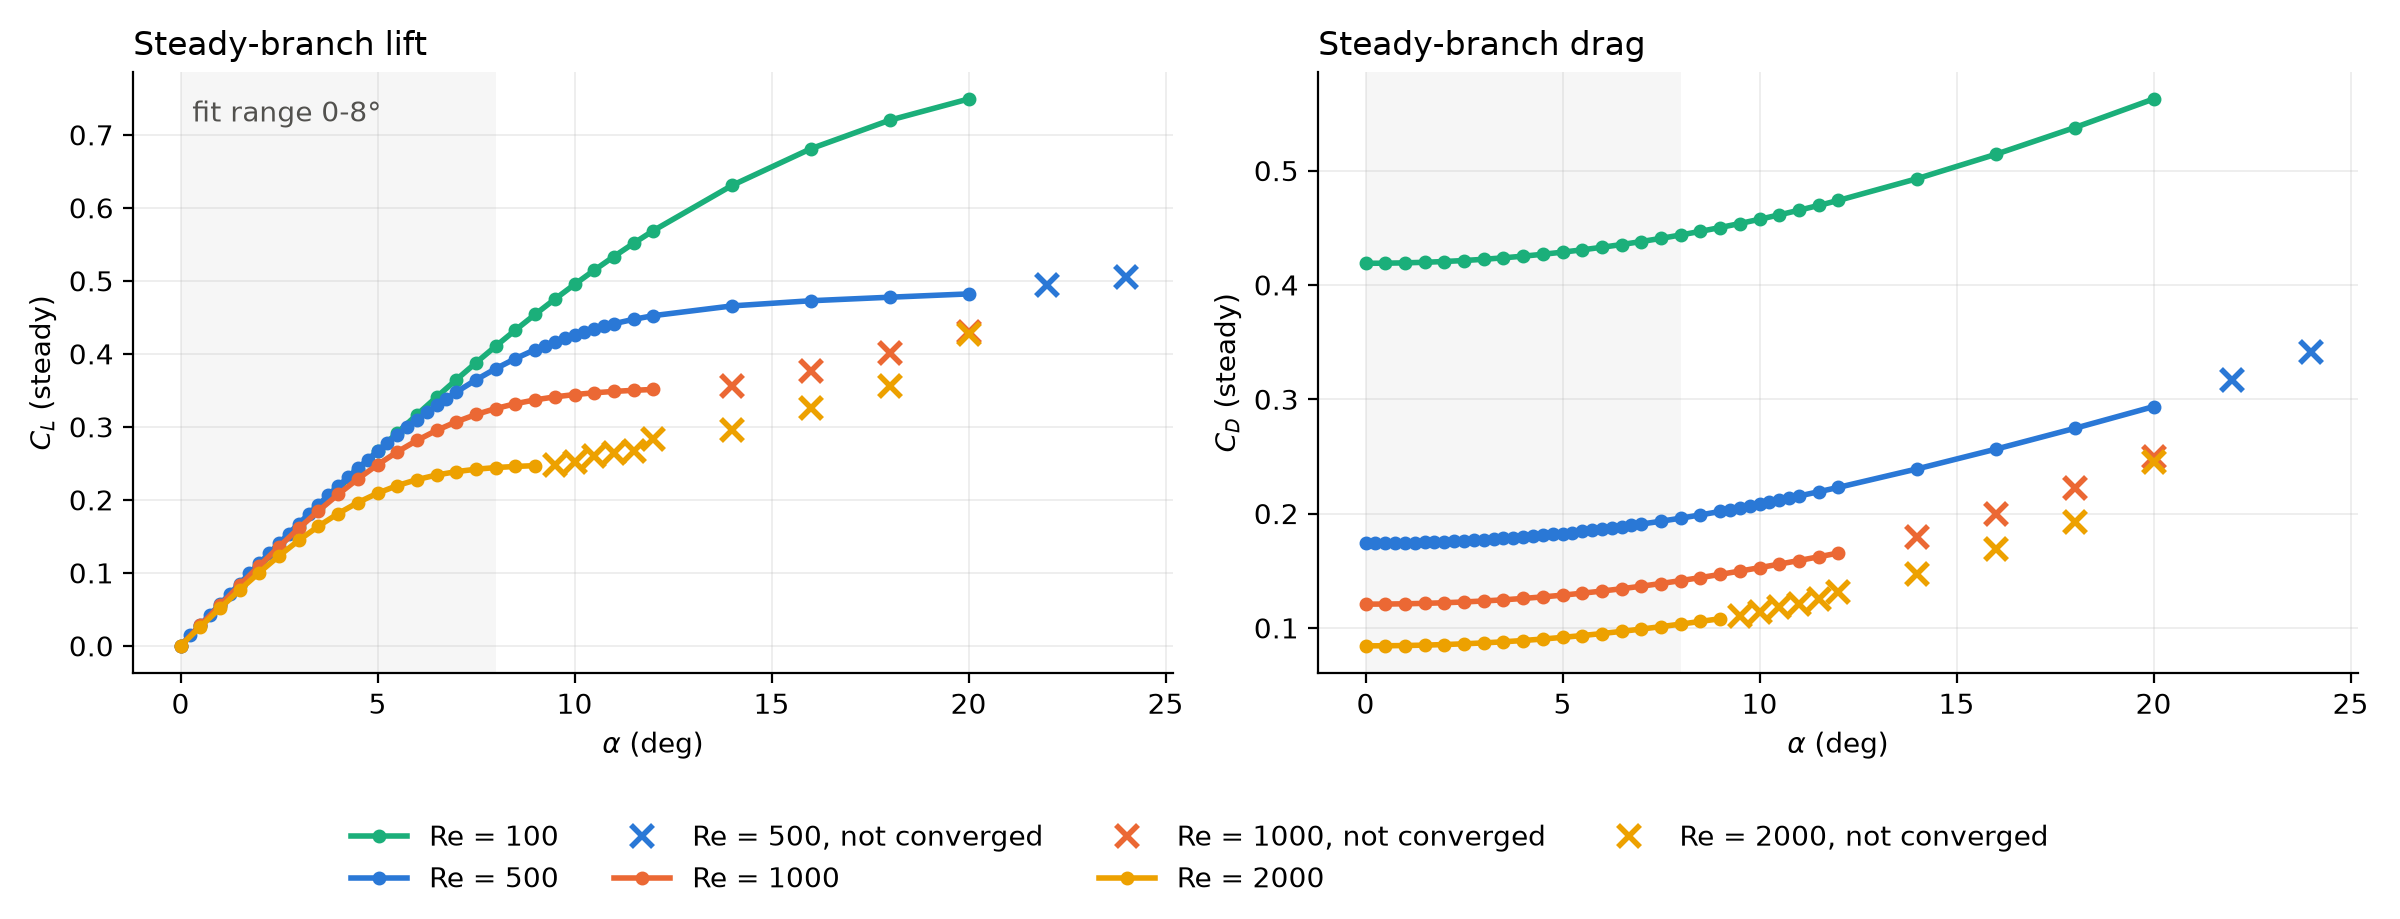
\includegraphics[width=\figw]{resweep_steady_0to8deg_odd/steady_lift_drag_re100_vs_re500_vs_re1000_vs_re2000.png}
\caption{Steady lift and drag. Dots: converged steady solutions. Crosses: the steady
solver did not settle (last iterate shown, not a solution). Shaded: fit range
$0$--$8^\circ$.}
\label{fig:lift}
\end{figure}

\begin{itemize}[leftmargin=*]
\item \textbf{All four curves start with the same slope}, about 3.1--3.3 per radian.
\item \textbf{They peel away in order of Re.} Re = 100 keeps climbing to $20^\circ$
  ($\CL = 0.75$). Re = 2000 is nearly flat from $7^\circ$ to $9^\circ$ (0.239 to 0.247).
\item \textbf{Drag falls about five-fold} from Re = 100 to Re = 2000, from 0.419 to
  0.084 at $0^\circ$.
\end{itemize}

\FloatBarrier
\subsection{Lasso, odd terms only, \texorpdfstring{$0$--$8^\circ$}{0-8 deg}}

\begin{table}[htbp]
\centering
\caption{Lasso at $\lambda = 10^{-4}$: coefficient of each (rescaled) term, with the
fraction of 500 bootstrap resamples that kept it in brackets.}
\begin{tabular}{lrrrr}
\toprule
term & Re 100 & Re 500 & Re 1000 & Re 2000 \\
\midrule
$\theta$   & $+0.131$ (1.00) & $+0.137$ (1.00) & $+0.134$ (1.00) & $+0.122$ (1.00) \\
$\theta^3$ & $-0.001$ (0.37) & $-0.017$ (0.97) & $-0.035$ (1.00) & $-0.054$ (1.00) \\
$\theta^5$ & $-0.005$ (0.98) & $-0.004$ (1.00) & $-0.0002$ (0.83) & $0$ (0.03) \\
$\theta^7$ & $0$ (0.10) & $0$ (0.00) & $0$ (0.00) & $0$ (0.00) \\
$\theta^9$ & $0$ (0.01) & $0$ (0.00) & $0$ (0.00) & $+0.004$ (0.89) \\
\bottomrule
\end{tabular}
\end{table}

\begin{itemize}[leftmargin=*]
\item \textbf{At Re = 500, 1000 and 2000}, $\theta$ and $\theta^3$ are firm choices.
  The $\theta^3$ coefficient grows steadily with Re.
\item \textbf{At Re = 100} the bend is so small that Lasso cannot tell $\theta^3$ from
  $\theta^5$.
\item \textbf{At Re = 2000} the $0$--$8^\circ$ range includes the flattening, so a high
  power ($\theta^9$) appears to absorb it. On $0$--$6^\circ$ it is $\theta + \theta^3$
  again.
\end{itemize}

\begin{figure}[htbp]
\centering
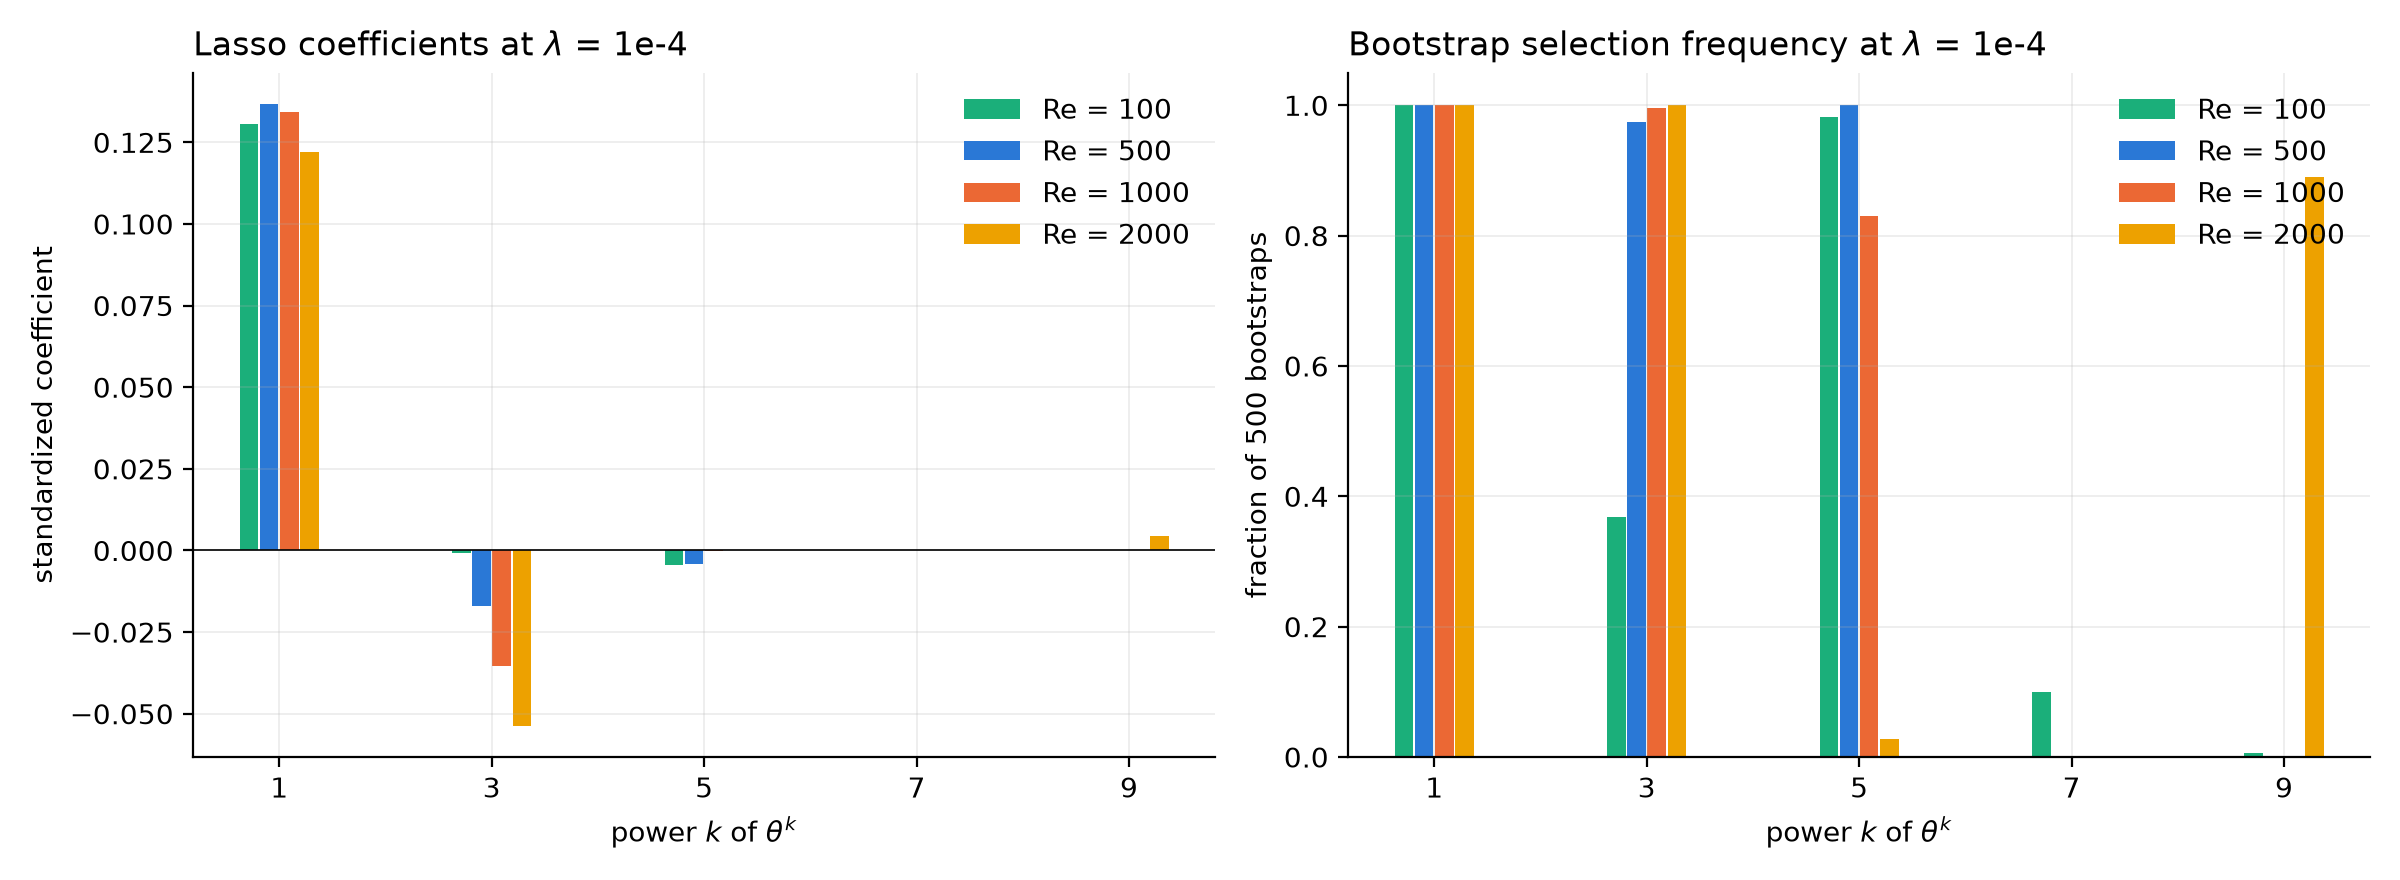
\includegraphics[width=\figw]{resweep_steady_0to8deg_odd/lasso_coefficients_re100_vs_re500_vs_re1000_vs_re2000.png}
\caption{Lasso coefficients (left) and how often each term survived resampling (right),
$0$--$8^\circ$.}
\end{figure}

\FloatBarrier
\subsection{Legendre coefficients}

\begin{table}[htbp]
\centering
\caption{Odd Legendre fit on $x = \theta/\theta_{\max}$, $\theta_{\max} = 8^\circ$,
mirrored to $[-1,1]$. RMSE is the typical leftover error in $\CL$.}
\small
\begin{tabular}{rrrrrrr}
\toprule
Re & $c_1$ & $c_3$ & $c_5$ & $c_7$ & $c_9$ & RMSE \\
\midrule
100  & $+0.42111$ & $-0.010754$ & $+9.7\times10^{-5}$ & $+2.4\times10^{-6}$ & $-6.5\times10^{-8}$ & $2.9\times10^{-8}$ \\
500  & $+0.41020$ & $-0.030895$ & $+2.6\times10^{-4}$ & $+1.4\times10^{-4}$ & $-1.6\times10^{-6}$ & $5.0\times10^{-7}$ \\
1000 & $+0.37164$ & $-0.048816$ & $+1.8\times10^{-3}$ & $+5.5\times10^{-4}$ & $-5.4\times10^{-5}$ & $2.8\times10^{-6}$ \\
2000 & $+0.30219$ & $-0.066533$ & $+8.3\times10^{-3}$ & $+6.9\times10^{-4}$ & $-4.1\times10^{-4}$ & $1.0\times10^{-5}$ \\
\bottomrule
\end{tabular}
\end{table}

\begin{itemize}[leftmargin=*]
\item \textbf{$c_1$ and $c_3$ carry the curve at every Re.} The bend relative to the
  straight part, $|c_3/c_1|$, is 2.6\,\%, 7.5\,\%, 13\,\% and 22\,\% from Re = 100 to
  2000.
\item \textbf{The finer terms shrink quickly at low Re and slowly at high Re.} At
  Re = 100 each step is about 100 times smaller. At Re = 2000, $c_5$ is still 12\,\% of
  $c_3$, so the third term is real there.
\item \textbf{The smallest coefficients are below the data's precision.} The lift is
  stored to about $10^{-7}$, so $c_7$ and $c_9$ at Re = 100 describe rounding, not flow.
\end{itemize}

\begin{table}[htbp]
\centering
\caption{Typical leftover error (RMSE in $\CL$) when the Legendre series is cut off
after a given term.}
\begin{tabular}{rccccc}
\toprule
Re & $P_1$ & $P_1$--$P_3$ & $P_1$--$P_5$ & $P_1$--$P_7$ & $P_1$--$P_9$ \\
\midrule
100  & $4.4\times10^{-3}$ & $3.4\times10^{-5}$ & $7.2\times10^{-7}$ & $3.4\times10^{-8}$ & $2.9\times10^{-8}$ \\
500  & $1.3\times10^{-2}$ & $1.1\times10^{-4}$ & $4.1\times10^{-5}$ & $6.6\times10^{-7}$ & $5.0\times10^{-7}$ \\
1000 & $2.0\times10^{-2}$ & $6.7\times10^{-4}$ & $1.6\times10^{-4}$ & $1.5\times10^{-5}$ & $2.8\times10^{-6}$ \\
2000 & $2.7\times10^{-2}$ & $2.9\times10^{-3}$ & $2.0\times10^{-4}$ & $1.1\times10^{-4}$ & $1.0\times10^{-5}$ \\
\bottomrule
\end{tabular}
\end{table}

\begin{figure}[htbp]
\centering
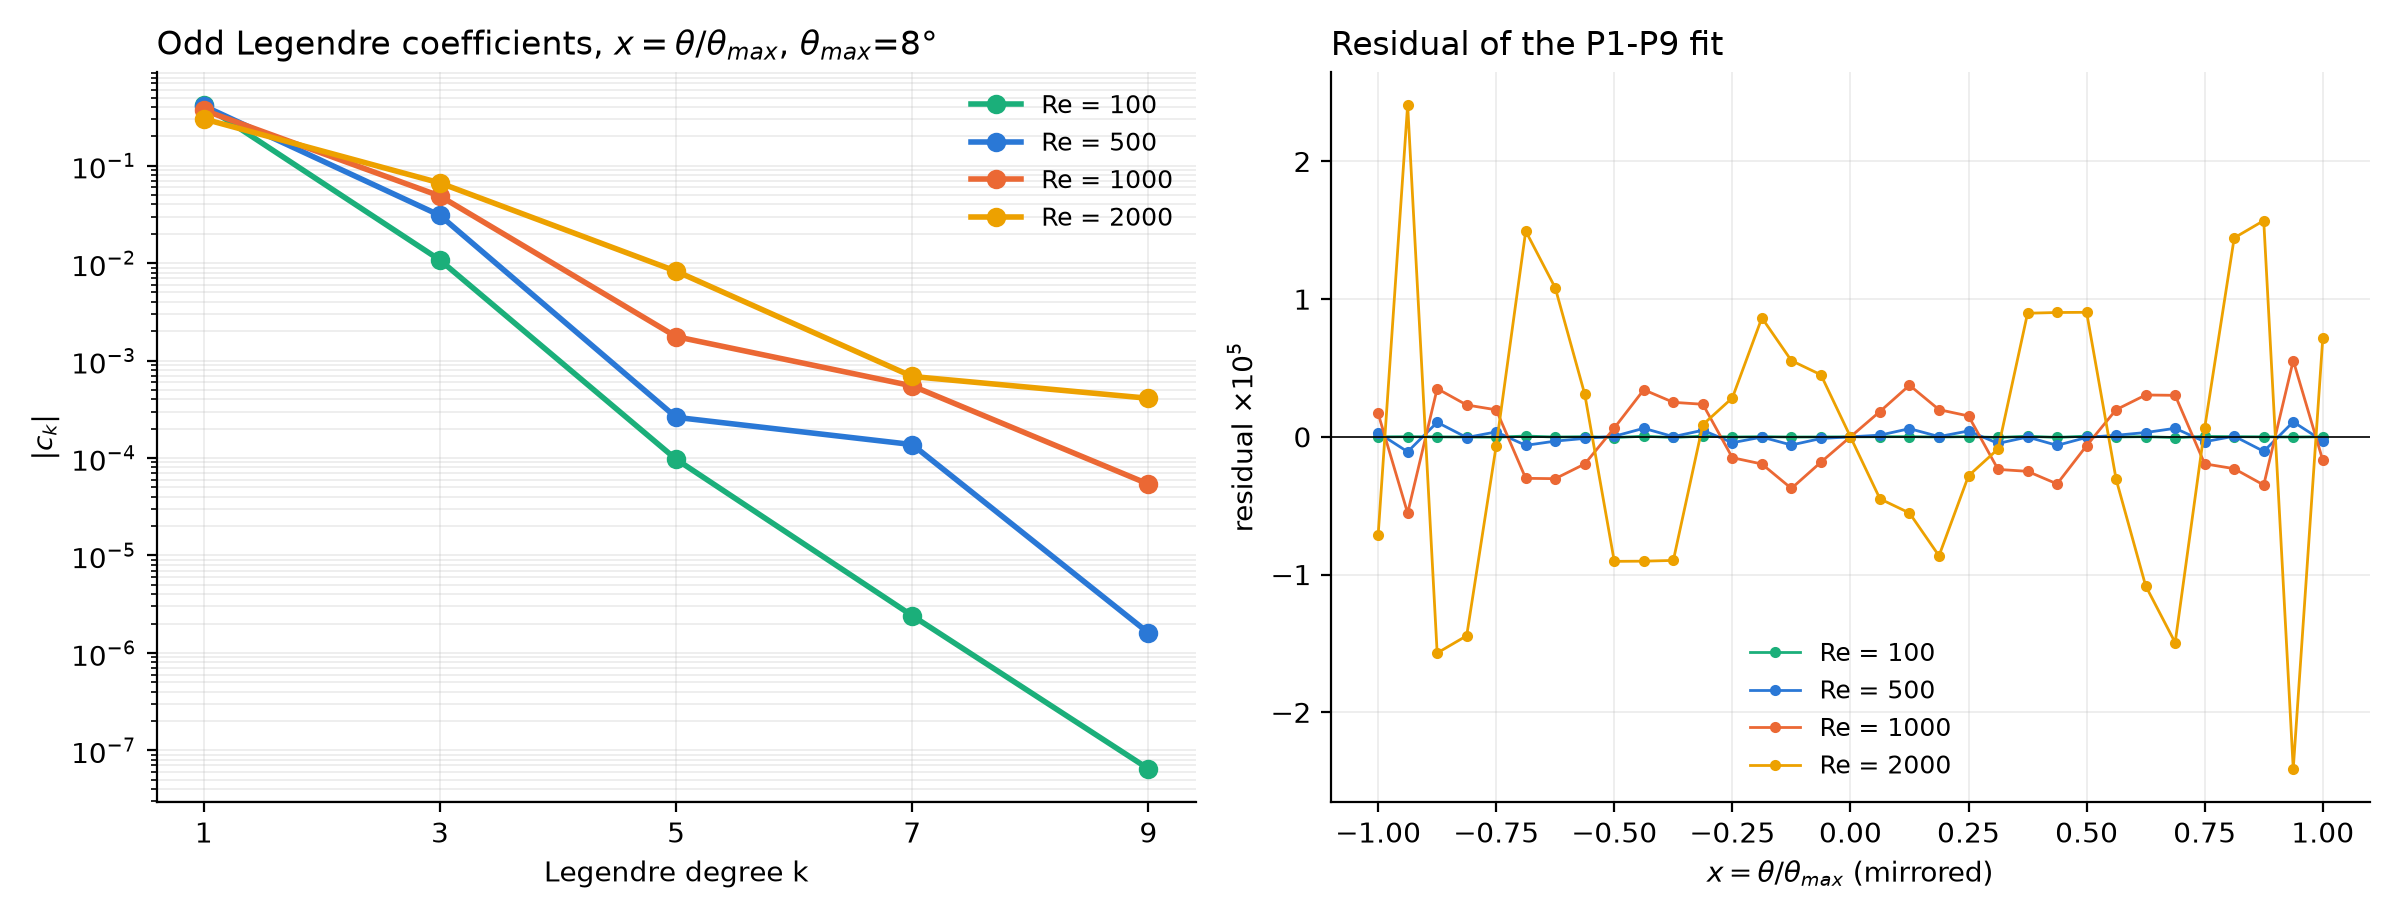
\includegraphics[width=\figw]{legendre_odd_0to8deg/legendre_odd_coeffs.png}
\caption{Left: size of each Legendre coefficient (log scale). A steep drop means the
series converges fast. Right: leftover error of the full five-term fit.}
\end{figure}

\FloatBarrier
\subsection{Back in powers of \texorpdfstring{$\theta$}{theta}}

\begin{table}[htbp]
\centering
\caption{The Legendre fits rewritten as $a_1\theta + a_3\theta^3 + a_5\theta^5$
($\theta$ in radians), cut off after $P_3$ or $P_5$.}
\begin{tabular}{rrrrr}
\toprule
Re & from & $a_1$ & $a_3$ & $a_5$ \\
\midrule
100  & $P_1$--$P_3$ & 3.131 & $-9.86$  & \\
500  & $P_1$--$P_3$ & 3.269 & $-28.30$ & \\
1000 & $P_1$--$P_3$ & 3.183 & $-44.41$ & \\
2000 & $P_1$--$P_3$ & 2.866 & $-59.56$ & \\
2000 & $P_1$--$P_5$ & 2.991 & $-87.84$ & $+1236$ \\
\bottomrule
\end{tabular}
\end{table}

\noindent
\textbf{The recommended model:}
\begin{itemize}[leftmargin=*]
\item \textbf{For Re $\le 1000$:} the two-term form $\CL = a_1\theta + a_3\theta^3$,
  accurate to $7\times10^{-4}$ or better.
\item \textbf{At Re = 2000:} keep the $\theta^5$ term (error $2\times10^{-4}$).
\end{itemize}

\noindent
\textbf{Do not take higher powers of $\theta$ at face value.} If all five Legendre terms
are rewritten in powers of $\theta$, the $\theta$ and $\theta^3$ parts stay put, but
$\theta^5$ to $\theta^9$ get huge coefficients of alternating sign that almost cancel
(Figure~\ref{fig:collected}). At Re = 2000 the $\theta^9$ coefficient comes out at
$-1.9\times10^{6}$. That is the look-alike problem of Section~\ref{sec:lookalike}
reappearing, not physics.

\begin{figure}[htbp]
\centering
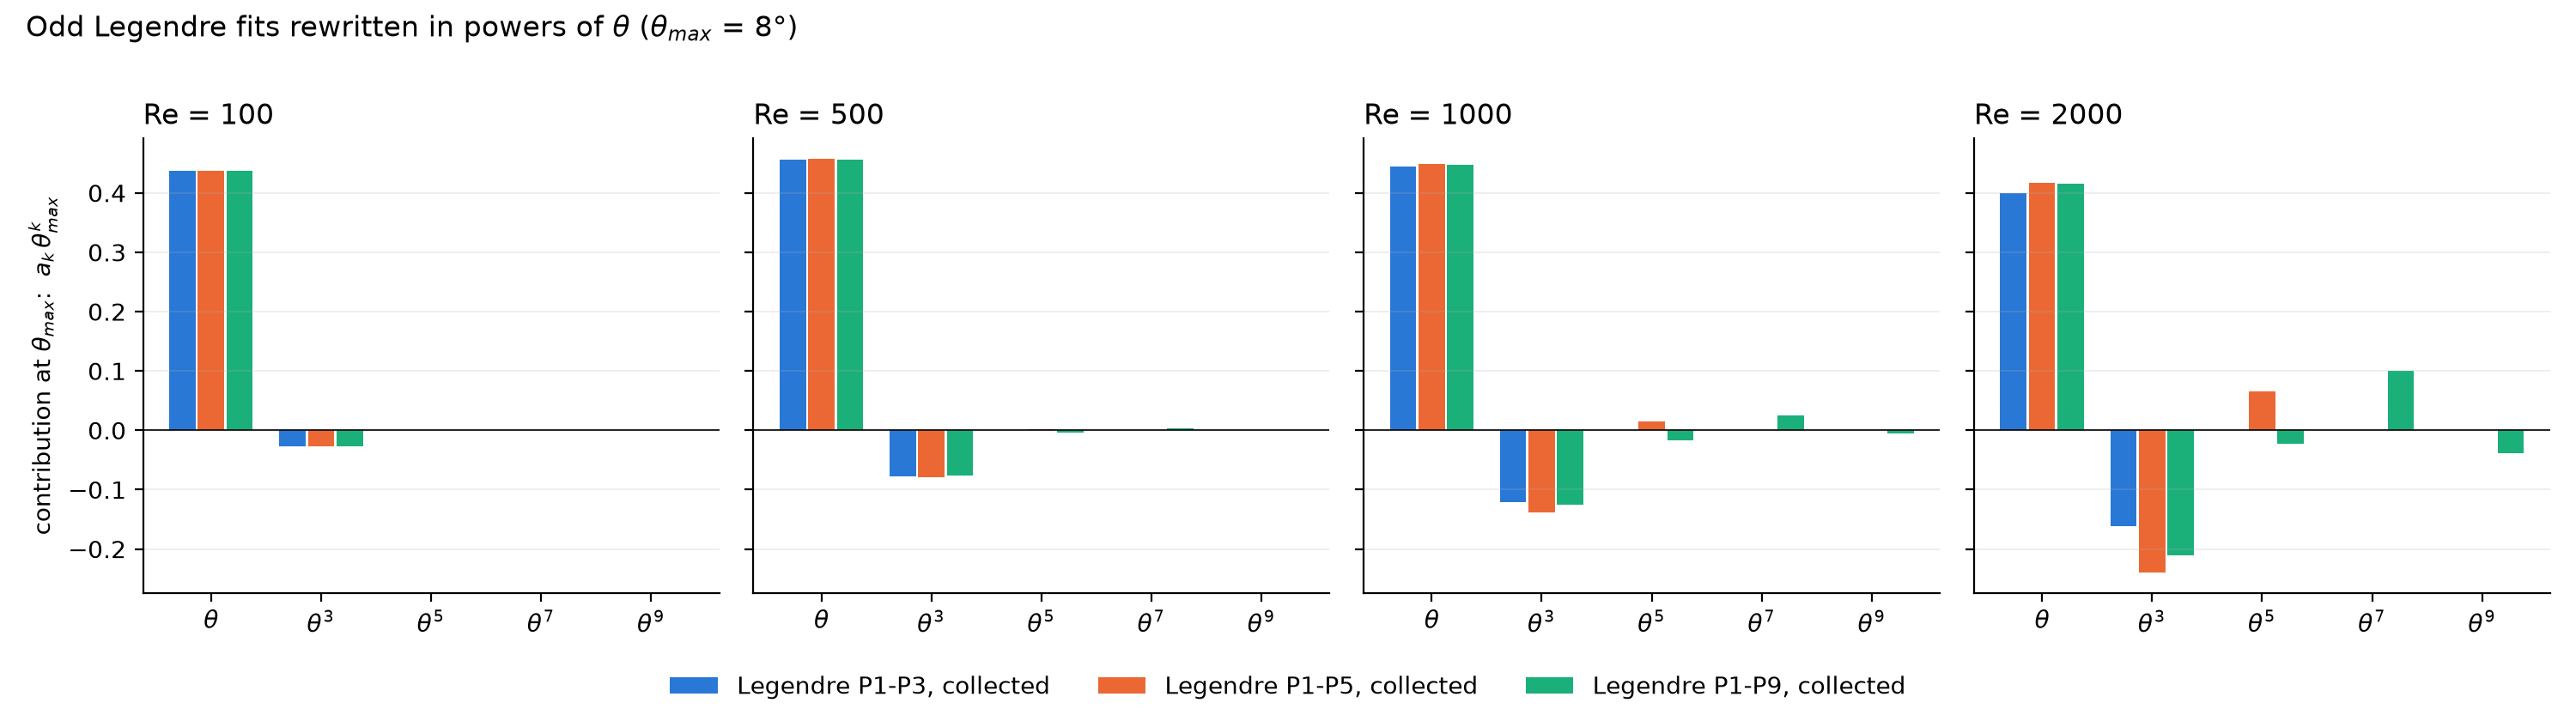
\includegraphics[width=\figw]{legendre_odd_0to8deg/theta_basis_collected.png}
\caption{Each power of $\theta$'s contribution to $\CL$ at $8^\circ$, after rewriting
the Legendre fits. $\theta$ and $\theta^3$ are the same whichever cut-off is used. The
higher powers change size and sign.}
\label{fig:collected}
\end{figure}

\FloatBarrier
\subsection{How the bend scales with Reynolds number}

\begin{figure}[htbp]
\centering
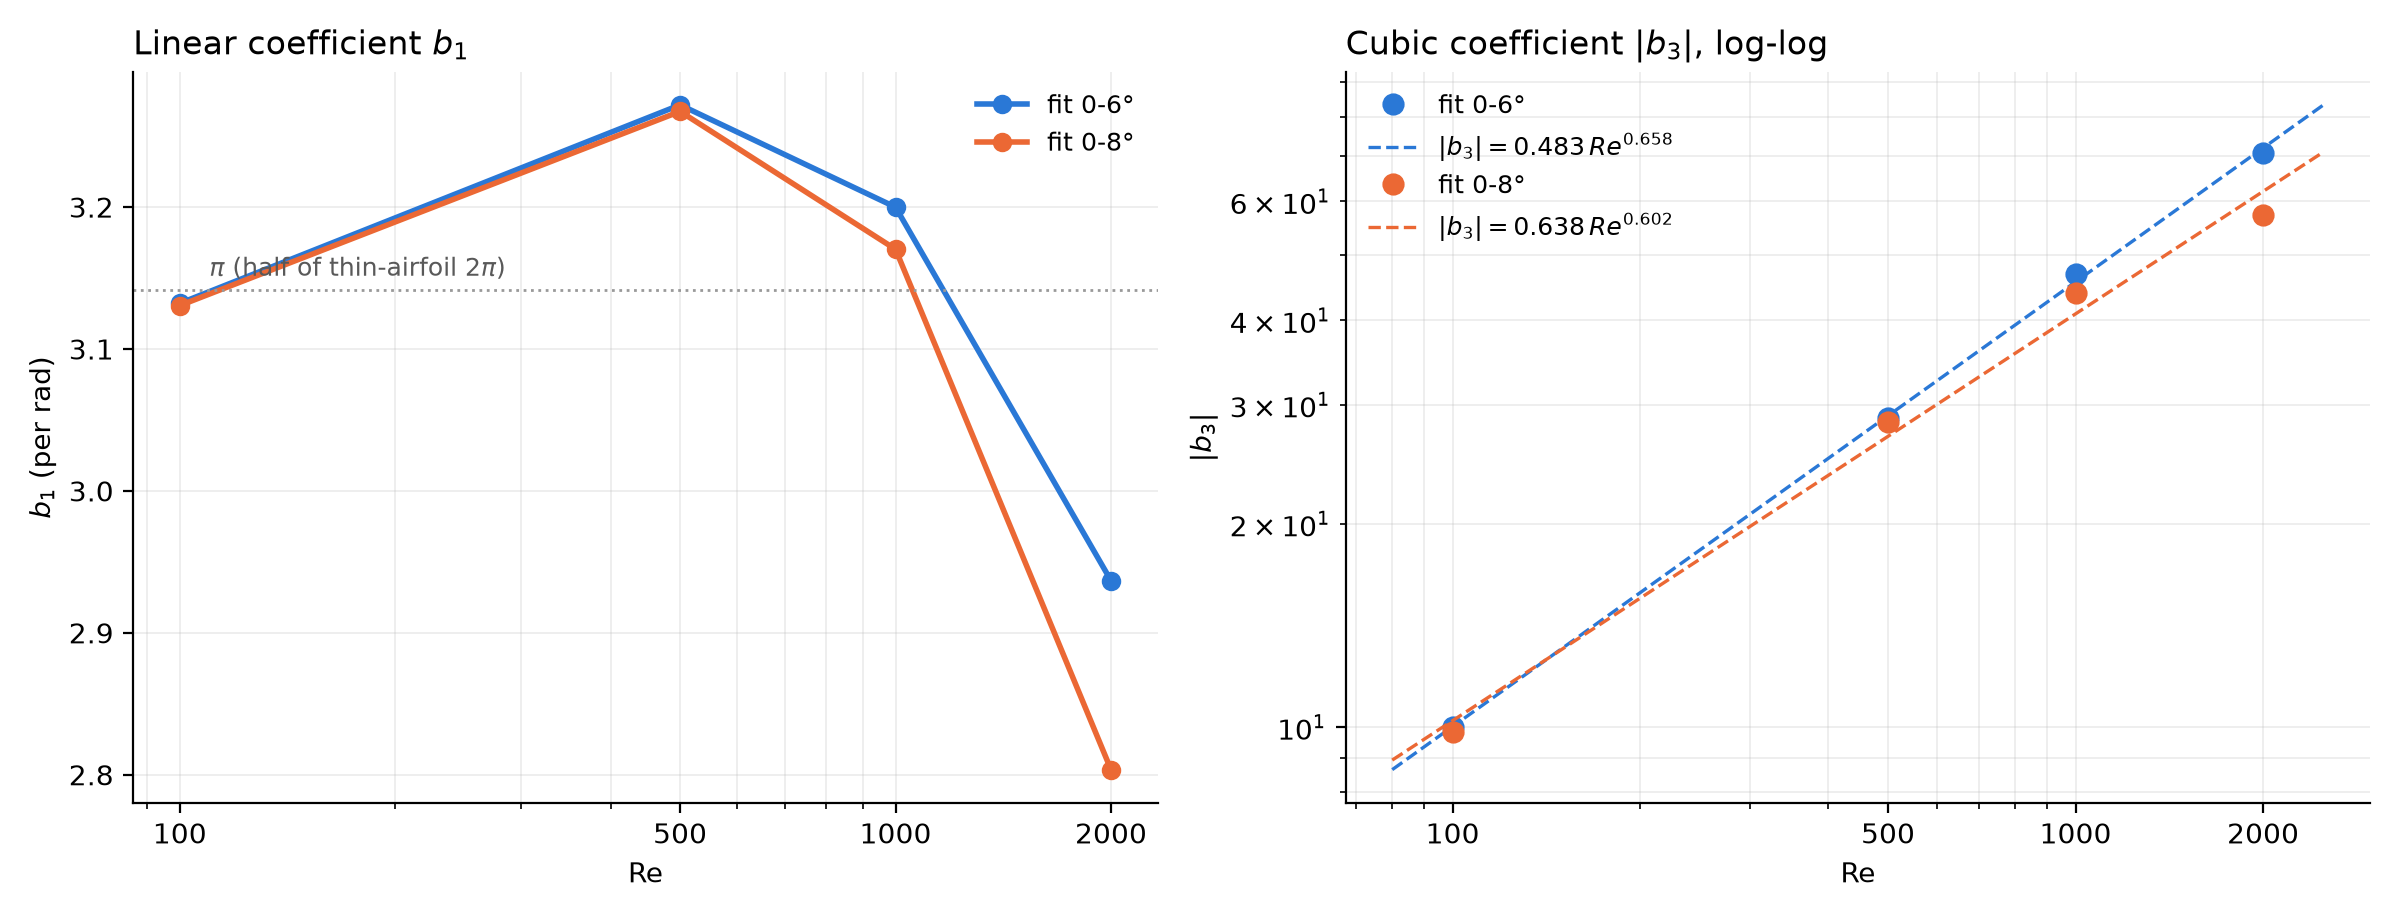
\includegraphics[width=\figw]{resweep_cubic_vs_re/cubic_coeffs_vs_re.png}
\caption{Two-term least-squares fit $b_0 + b_1\theta + b_3\theta^3$ at each Re. Left:
linear coefficient $b_1$, near $\pi$. Right: $|b_3|$ on log--log axes, with a power-law
fit for two fit ranges.}
\end{figure}

\begin{itemize}[leftmargin=*]
\item \textbf{The fit:} $|b_3| = 0.48\,\mathrm{Re}^{0.66}$ over $0$--$6^\circ$, with
  every point within about 3\,\% of the line.
\item \textbf{The $0$--$8^\circ$ version is less clean:} $0.64\,\mathrm{Re}^{0.60}$.
  Its Re = 2000 point already includes the flattening of the curve.
\item \textbf{A candidate model to test, not a result:}
  $\CL(\theta, \mathrm{Re}) \approx b_1\theta - 0.48\,\mathrm{Re}^{0.66}\theta^3$.
\end{itemize}

\FloatBarrier
\subsection{Unsteady check at Re = 2000, \texorpdfstring{$9.5^\circ$}{9.5 deg}}
\label{sec:unsteady}

\begin{figure}[htbp]
\centering
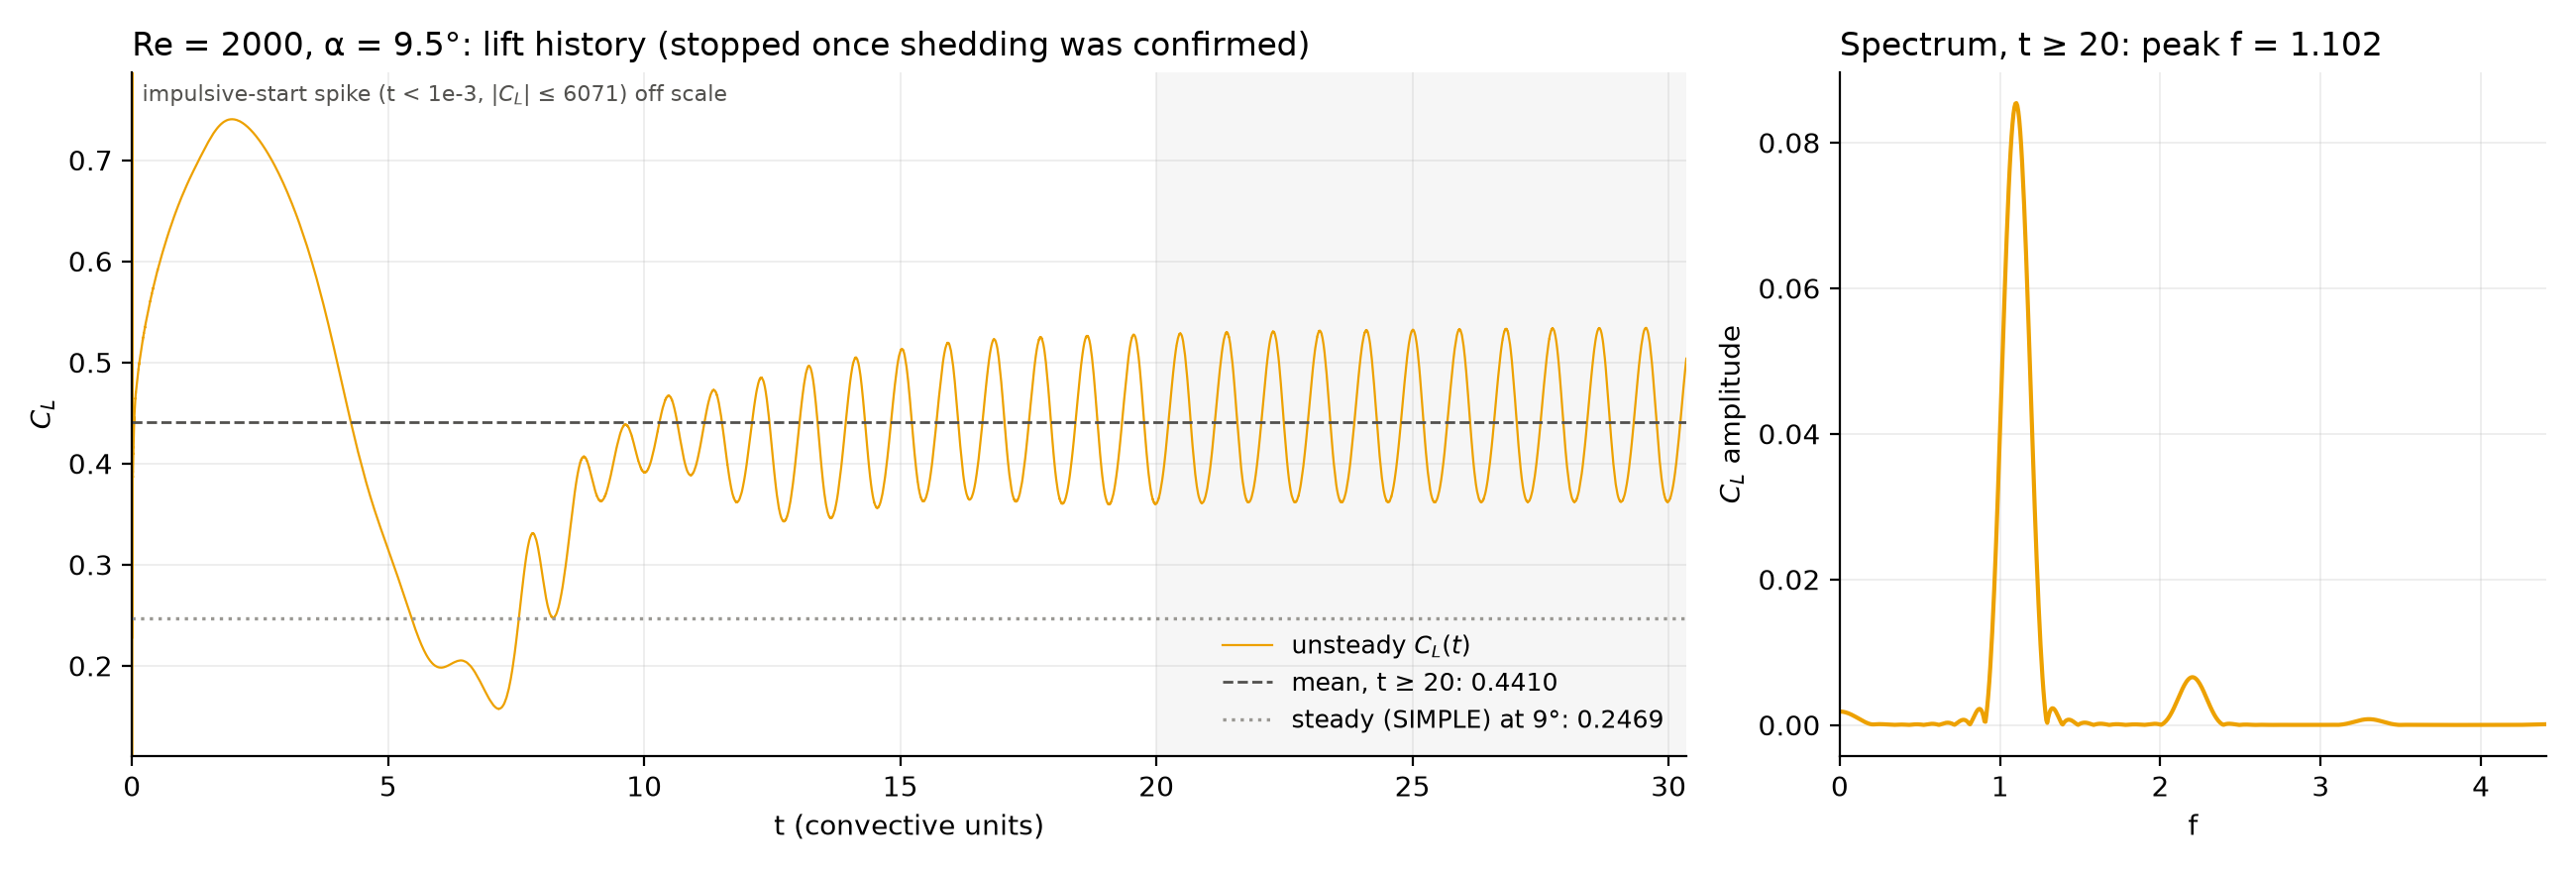
\includegraphics[width=\figw]{unsteady_re2000/cl_aoa9.5.png}
\caption{Time-accurate lift at Re = 2000, $\alpha = 9.5^\circ$ (left) and its frequency
content after $t = 20$ (right). The very large start-up spike in the first $10^{-3}$
time units is off scale.}
\end{figure}

\begin{itemize}[leftmargin=*]
\item \textbf{Shedding starts at $t \approx 8$} and settles into a steady oscillation by
  $t \approx 20$.
\item \textbf{It is a clean single-frequency oscillation:} $f = 1.10$, with only
  harmonics at $2f$ and $3f$.
\item \textbf{It does not die out.} The oscillation envelope is flat to very slowly
  growing.
\item \textbf{$\CL = 0.441 \pm 0.087$.} Even the lowest point of the cycle, 0.361, is
  above the steady value of 0.247. The real flow does not oscillate \emph{around} the
  steady solution; it lives somewhere else entirely. We saw the same picture at
  Re = 500.
\end{itemize}

\FloatBarrier
\clearpage
\section*{Where things are}

\begin{itemize}[leftmargin=*]
\item \textbf{Cases:} \texttt{steady\_re\{100,500,1000,2000\}/} and
  \texttt{unsteady\_re2000/re2000\_aoa9.5/}.
\item \textbf{Fitting scripts:} \texttt{analysis/lasso\_re1000.py} (Lasso),
  \texttt{analysis/legendre\_odd\_fit.py} (Legendre), \texttt{analysis/cubic\_vs\_re.py}
  (power law).
\item \textbf{Figures:} \texttt{analysis/explain\_figs.py} and
  \texttt{analysis/plot\_unsteady\_re2000.py}.
\item \textbf{Full technical record:} \texttt{STEADY\_LASSO\_Re1000.md} and
  \texttt{STEADY\_LASSO\_ReSweep.md}.
\end{itemize}

\end{document}
